\documentclass[conference]{IEEEtran} % onecolumn
\usepackage{cite}
\usepackage{amsmath,amssymb,amsfonts}
\usepackage{algorithmic}
\usepackage{graphicx}
\usepackage{textcomp}
\usepackage{xcolor}
\usepackage{float}
\usepackage{booktabs}
\usepackage{pxfonts}
\usepackage{listings}
\usepackage{epstopdf}

\def\BibTeX{{\rm B\kern-.05em{\sc i\kern-.025em b}\kern-.08em
    T\kern-.1667em\lower.7ex\hbox{E}\kern-.125emX}}
    
% Define standard verbatim listing style
\lstdefinestyle{standard}{
  basicstyle=\fontsize{9}{9}\ttfamily,
  columns=flexible,
  breaklines=true,
  escapechar=\#
}

\newcommand{\mytilde}{\raise.17ex\hbox{$\scriptstyle\mathtt{\sim}$}}


\begin{document}
\title{Generic Data Broadcast using Bluetooth Low Energy Advertisement Packets\\
}

\author{\IEEEauthorblockN{\textbf{David Jones}}
\IEEEauthorblockA{\textit{School of Electronics and Computer Science} \\
\textit{University of Southampton}\\
Southampton, United Kingdom \\
dsj1n15@ecs.soton.ac.uk}
\and
\IEEEauthorblockN{Richard Crosland}
\IEEEauthorblockA{\textit{School of Electronics and Computer Science} \\
\textit{University of Southampton}\\
Southampton, United Kingdom \\
rtc1g16@ecs.soton.ac.uk}
}
\maketitle

\begin{abstract}
Bluetooth is a ubiquitous communications technology present in billions of devices worldwide. While proximity based content delivery methods often rely on end-device internet connections to carry out data transfer, this article describes an approach for achieving offline and connectionless data broadcasts using Bluetooth Low Energy (BLE) advertisement packets. The resulting protocol has an effective concurrent transfer rate of 0.06kB/s to each receiver. Although low-rate, the system is unaffected by receiver count. While BLE is fundamentally low-power and transmission duty cycle is consistent between the proposed approach and other beacon services (e.g. Apple's iBeacon), the encoding procedure means that more complex beacon hardware may be required.
\end{abstract}

\begin{IEEEkeywords}
BT, LE, BLE, Beacon, Broadcast, Lossy, Luby-Transform, Fountain Codes
\end{IEEEkeywords}

\section{Introduction}
Bluetooth\footnote{Bluetooth SIG, USA, https://www.bluetooth.com} is a short-range, single-hop communication technology, which as of 2019, is present in 100\% of shipped smartphones, tablets, and laptops \cite{BT:MARKET_RESEARCH}. Since 2010, implementations typically utilise Bluetooth v4.0 or newer; this packages Bluetooth Low Energy (BLE) alongside traditional (Classic) Bluetooth (BT) \cite{BT:CORE_SPEC}. This opens up mobile devices to proximity based content delivery services, such as: Apple's iBeacon\footnote{Apple, USA, https://developer.apple.com/ibeacon/}, Google's Eddystone\footnote{Google, USA, https://developers.google.com/beacons/eddystone} and and Radius Network's AltBeacon\footnote{Radius Network, USA, https://altbeacon.org}. These are used in many industries but are most prevalent in advertising for purposes such as tracking in-store shoppers \cite{BT:TRACK_USE_CASE}, and serving offers directly. Typically, content delivery implementations are backed by an internet server, allowing the beacon to transmit only a unique identifier (UUID), for which the target device can then download the corresponding payload. This allows beacons to operate completely offline and use minimal power, but limits deployments to locations where end-user's have a reliable internet connection. For purposes such as advertising, this connection would ideally be served by cellular LTE, though this can be unreliable indoors, whilst relying on users to connect to in-store Wi-Fi reduces potential catchment.

This article assesses whether small-medium payload broadcasting is viable using a BLE beacon approach without a second transfer medium. The use of fountain codes is explored as a way of coping with the unpaired lossy connection. 
%A brief use case is also trialled using a custom data structure for generating offline advertisements.

\section{Background}
\subsection{Bluetooth Low Energy (BLE)}
As its namesake suggests, BLE has significantly lower power usage than BT to the point it can operate in an always-on fashion with minimal effect to the end-user -- the drawback being an overall lower achievable data-rate. This is achieved from a physical layer standpoint as well as the introduction of a simplified protocol stack; as shown in Fig. \ref{fig:bt_stack}. 


\begin{figure}[H]
    \centering
   	\includegraphics[scale=0.75]{Figures/bt_stack}
    \caption[Bluetooth network stack]{
  The BLE network stack adapted from \cite{BT:LE_OVERVIEW}. 
    }
    \label{fig:bt_stack}
\end{figure}

Most BLE applications involve connecting multiple peripheral devices to a single device (the central), for example, connecting a heart-rate monitor and smartwatch to a mobile phone. This allows moderate one-to-one data transfer rates of approximately 125kB/s \cite{BT:LE_OVERVIEW}. These dedicated connection scenarios are handled by the Generic Attribute Profile (GATT). As communications that occur here are only visible by the intended receiver, broadcast is not possible. For sending small identical payloads to many receivers, this significantly increases network congestion and collisions associated with dense wireless environments. 

The Generic Access Profile (GAP) manages device advertisements and connections to nearby devices. Advertisements occur at frequent intervals or when a Scan Response Request is received from another device. Each Bluetooth Advertising Protocol Data Unit (PDU) has 31 bytes of data that can be set by the transmitter -- the rest being reserved for the BLE stack. By default these advertisements are sequentially transmitted to three BLE channels. These channels are selected away from standard 2.4GHz Wi-Fi channels to reduce potential interference, giving higher receive probabilities than other BLE transmissions. An advertisement can be either directed (unicast) or undirected (broadcast), and either connectable or non-connectable. Advertisements are the only place broadcast communications can occur and are the basis for beacon operation. As connecting defeats the purpose of broadcast behaviour, beacons are non-connectable. As specified by \cite{BT:CORE_SPEC}, non-connectable advertisements (\texttt{ADV\_NONCONN\_IND}) should be limited to transmission every 100ms unlike connectable advertisements (\texttt{ADV\_IND}) which can be sent every 20ms.

\subsection{BLE Beacons}
Although frame structures vary slightly and Eddystone beacons have some extra functionality, the fundamentals of all pre-mentioned beacon implementations are very similar. That is: periodically send BLE advertisements with some payload packaged in the manufacturer data section -- see Fig. \ref{fig:altbeacon_frame} for AltBeacon's standard payload. An application must be installed on the receiver to interpret and handle the received payload.

\begin{figure}[H]
    \centering
   	\includegraphics[scale=0.75]{Figures/altbeacon_frame}
    \caption[Altbeacon frame]{
  An AltBeacon frame. Note that 3 bytes of the manufacturer data are used to indicate that the advertisement is non-connectable and undirected hence making the maximum payload 28 bytes, not 31. Additionally, some fields are fixed. AD length is \texttt{0x1B} (27) to indicate the payload size. AD Type is set to \texttt{0xFF} to indicate that the frame is manufacturer data and should not be handled by the stack. The Beacon Code is \texttt{0xBEAC} to identify the frame as an AltBeacon. The rest of the fields values can change. The Manufacturer ID identifies the transmission hardware as per Bluetooth SIG company identifiers. The Beacon ID uniquely identifies the transmitter. The Reference RSSI is the received signal strength 1m away from the transmitter to allow for distance estimates. The Manufacturer Data is interpreted as defined by the Manufacturer ID but is generic. The manufacturer data is little endian whereas the rest is big endian. Adapted from \cite{BT:ALTBEACON}.
    }
    \label{fig:altbeacon_frame}
\end{figure}

\section{Test/Development Infrastructure}
The testing and development platforms used for the findings of this article were as follows:
\begin{itemize}
	\item \textbf{Beacons:} Raspberry Pi 3's (Model B+) running Raspian OS; these have built-in BT v4.2 and the operating system provides BlueZ\footnote{BlueZ Project, http://www.bluez.org}, which directly exposes the Host-Controller Interface (HCI) as identified in Fig. \ref{fig:bt_stack}. The command line tool was scripted using a Python wrapper.
	\item \textbf{End-devices:} Android smartphones, specifically the OnePlus X (BT v4.0) and Samsung S8 (BT v5.0). A bespoke application was developed with the Android Beacon Library\footnote{Radius Networks, USA, https://altbeacon.github.io/android-beacon-library/} providing the basis of BT interaction.
\end{itemize}

Beacon advertisements were set to occur at their fastest rate, every 100ms. 
%The BT setup commands were as follows (refer to \cite{BT:CORE_SPEC} for full command breakdowns):
%\begin{lstlisting}[style=standard]
%// Enable the BT interface
%$ hciconfig up
%// Disable scanning for other devices, transmit only
%$ hciconfig noscan
%// CMD : LE Set Advertising Parameters [p. 1321]
%// (set to 100ms period) 
%$ hcitool cmd 0x08 0x0006 A0 00 A0 00 03 00 00 00 00 00 00 00 00 07 00
%// CMD : LE Set Advertising Enable [p. 1329]
%// Enable non-connectable undirected advertising
%$ hcitool cmd 0x08 0x000a 01
%\end{lstlisting}
%After setup, the periodically transmitted data could be set with the following command:
%\begin{lstlisting}[style=standard]
%// CMD : LE Set Advertising Data [p. 1326]
%$ hcitool cmd 0x08 0x0008 {ADVERTISING_BYTES}
%\end{lstlisting}
Likewise the Android Beacon Library was configured to receive as frequently as possible using a 50ms search period and 0ms between search periods.


\section{Advertisement Receive Testing}
To determine whether data broadcast using advertisement packets was viable, initial assessment of the receive probability for each packet was required. This was handled by sending typical AltBeacon frames with the Beacon ID holding a basic test payload -- the top 8 bytes a constant pattern identifying test packets and the rest an incrementing packet count. The end-device reported the number of unique packets received as $n_{got}$. Tests transmitted 1000 packets ($n_{expected}$), after which an impression of receive probability could be calculated as $n_{got} / n_{expected}$. The packet transmissions were repeated until every unique packet had been received, $n_{repeats}$ giving  an indication of how many times a data payload would need to be retransmitted to ensure a single receiver gets the payload in the presence of no error correction. Of course, with the same packets being retransmitted, already received packets can be received again -- a clear waste of bandwidth. The results of performing the test 5 times are shown in Table \ref{tab:receive_prob}.
\begin{table}[H]
\caption{Test advertisment receive results}
\begin{center}
\begin{tabular}{c|ccccccccc}
\toprule
   & \multicolumn{9}{c}{\textbf{Repetition}} \\
\textbf{Test} & 1 & 2 & 3 & 4 & 5 & 6 & 7 & 8 & 9 \\
\midrule\addlinespace
1 & 556 & 834 & 960 & 992 & 998 & 998 & 999 & 999 & 1000 \\
2 & 440 & 796 & 944 & 987 & 999 & 1000 & - & - & -  \\
3 & 523 & 853 & 931 & 987 & 998 & 1000 & - & - & - \\
4 & 502 & 764 & 872 & 989 & 992 & 996 & 999 & 999 & 1000 \\
5 & 610 & 860 & 988 & 997 & 997 & 999 & 1000 & - & -  \\
\addlinespace\bottomrule
\end{tabular}
\end{center}
\label{tab:receive_prob}
\end{table}
 An average receive probability of 53\% ($p$) was found during the first transmission set with 9 repetitions required in the worst-case to receive all packets. With acknowledgment-retransmission mechanisms not possible in a unidirectional broadcast system, full payload delivery must either be handled by repeating transmissions or error correction.
\section{Protocol Proposal} 
A method for implementing efficient offline broadcasts is now proposed. The three main components are: a custom beacon payload format that maximises user data, a way of reducing the dependency on receiving every unique packet and a construction/deconstruction process for transmitted/received data.
\subsection{Beacon Frame}
The proposed frame format for broadcast data is detailed in Fig. \ref{fig:data_broadcast_frame}. The presence of the first four frame fields ensures the type can be used alongside existing beacon protocol types and is not limited to specialised beacon hardware. 
\begin{figure}[H]
    \centering
   	\includegraphics[scale=0.75]{Figures/data_broadcast_frame}
    \caption{
  Custom frame format for data broadcasts. Fields are defined the same as AltBeacon frames, however, the Beacon Code uses a different constant (\texttt{0xB0DC}) to identify the frame as a Data Broadcast Frame so that it is not mishandled. The MFG RSVD field is combined with the Beacon ID field to give 21 bytes of user data.
    }
    \label{fig:data_broadcast_frame}
\end{figure}

\subsection{Encoding/Packing}
The small size of the data portion means that many packets are required for sending any meaningful data. As there is no control over which packets are received, ideally the end-device should be able to receive a random scattering of packets and be able to reconstruct the data; this is the purpose of fountain codes. Although Raptor codes are theoretically the best (offering linear decoding time), this proof of concept uses the Luby Transform (LT) code. The reader is referred to \cite{BT:LUBY_TRANSFORM} for full algorithm details; a basic overview follows. The input data is split into $K$ fixed size blocks of $n$ bytes. Random selections of these blocks are XOR'd together to create encoded-blocks where the block count, called the degree ($d$), is also randomly decided. The pseudo random number generator (PRNG) seed used for generating each encoded-block, is transmitted with the block so that the decoder can determine the exact block generation criteria by seeding an identical PRNG. The decoder XORs known blocks (those with $d=1$) with unresolved blocks $d > 1$, reversing the encoding process, until all blocks are decoded (have $d=1$). $K'$ combined-blocks are required to decode where $K'$ is slightly more than $K$. At minimum $K' / p$ encoded-blocks should be transmitted, although as there are near-infinite encoded-blocks possibilities, any number of packets can be sent (he algorithm is rateless). The frame used for blocks is defined in Fig. \ref{fig:block_frame}. 

\begin{figure}[H]
    \centering
   	\includegraphics[scale=0.75]{Figures/block_frame}
    \caption{
   Structure for holding block data. Note that the Data Size field being 2 bytes limits broadcasts to 65,535 bytes, however, with each packet being limited to 10 bytes of actual payload, transmitting more is unlikely to be viable either way.
    }
    \label{fig:block_frame}
\end{figure}

A further header is attached to the Block Frame to form a Partial Chunk Frame (Fig. \ref{fig:partial_chunk_frame}). It holds: a Chunk ID that locally identifies the data group the block belongs to and a checksum formed from the bottom 16 bits of the frame's 32 bit CRC with an added nonse. The nonse is a constant (e.g. \texttt{0xB0DC}) added to the encoder version number \texttt{0xMMmm} where \texttt{M} is major and \texttt{m} is minor; ensuring decoders do not attempt to handle data that could have a different format to expected. 

\begin{figure}[H]
    \centering
   	\includegraphics[scale=0.75]{Figures/partial_chunk_frame}
    \caption{
    Structure that holds part of a chunk payload. 
    }
    \label{fig:partial_chunk_frame}
\end{figure}

Even with the Partial Chunk Frame's checksum, it is possible, though unlikely, that a rogue packet gets incorporated into the decoding process. Therefore decoded data must be verifiable, to this end a 32 bit CRC is calculated across the full payload and forms part of the Chunk Payload (Fig. \ref{fig:chunk_payload}). If CRC verification fails a different subset of received blocks can be used for decoding, or the full receive process can be reattempted. Of course, being broadcast data with no accountability or encryption, the payload must be handled with extreme care.

\begin{figure}[H]
    \centering
   	\includegraphics[scale=0.75]{Figures/chunk_payload}
    \caption{
    Wrapper for a payload so that it can be sent as a \textit{chunk}.
    }
    \label{fig:chunk_payload}
\end{figure}

Note that the defined structures are designed as a flexible proof of concept, potential payload could be increased by fixing certain values (e.g. block size) to remove unnecessary fields -- each header byte saved increases packet payload by 10\%.

\subsection{Process Overview}
\noindent \textbf{Beacon:}\\
\textit{Setup:} Takes in broadcast data, wraps it as a chunk and splits it into blocks (padded if necessary). 
\\ \textit{Loop:} From the blocks creates a new LT encoded-block, wraps it in the defined frames, sets it as the advertisement data, waits until the next advertisement.

\noindent \textbf{End Device:}\\
\textit{Loop:} Waits for data broadcasts frames to be present in advertisement packets, follows the verification procedure, assigns the encoded-block to the chunk's decoder. When enough data has been received and the decoder returns a result, the payload is verified using the CRC and handled as per the payload type.


\section{Implementation}
Other than the aforementioned BT handling methods and standard framing methods, the other major component of the implementation was the LT encoder/decoder. Encoding was handled using the lt-code\footnote{Anson Rosenthal, https://github.com/anrosent/LT-Code} Python library, with some modifications to handle custom header types (the block size, data size, and seed use 12 bytes by default, a large and unnecessary portion of the payload). The Android end-devices required a decoder, but as no Java solution was available, a manual Java translation was carried out for the library; this involved creating both the PRNG and block resolver. 

To be able to receive packets on the devices a custom AndroidBeaconLibrary parser for the Data Broadcast Frame was implemented: \lstinline[style=standard]{m:2-3=b0dc,i:4-24,p:25-25}. 

\section{Protocol Testing}
Testing was carried out using three different payload sizes: [A] 100B ($K=11$), [B] 1000B ($K=101$) and [C] 10,000B ($K=1001$). For perspective these could be considered as: a fully defined URL, a long text message (1000 characters) and a small bitmap image respectively. The beacon continuously transmitted encoded blocks with the receiver enabled at a random point in the stream. The receive times for 5 separate transmissions of each payload are plotted in Fig. \ref{fig:receive_time_plot}. The average receive times A, B, C respectively are: 2s, 17s and 149s -- indicating effective throughputs of: 0.05kB/s, 0.06kB/s, 0.06kB/s.
 
\begin{figure}[H]
    \centering
   	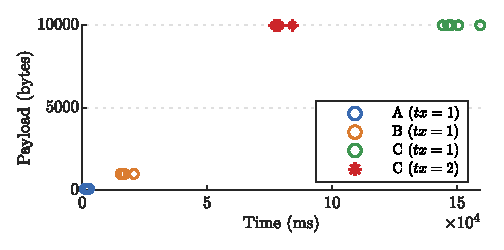
\includegraphics{Figures/networking_plot}
    \caption{
    Plot of receive times for differing payloads. The overall low-variance between results is clear with a linear correlation between payload size and transmission time -- both indicating reliable, consistent performance.
    }
    \label{fig:receive_time_plot}
\end{figure}

Also plotted are receive times for C where two beacons are simultaneously broadcasting the same payload, using the same Chunk ID, but different encoded-blocks. The average receive time in this case is 79s, 53\% of that with one transmitter; resulting in throughput of 0.12kB/s. Not only does this show that the system is handicapped by the high transmission interval (100ms) but also that data can be aggregated from multiple sources at once. This has potential applications in real-world environments such as scattering transmitters over large retail stores, increasing user exposure time and receive performance. 

For A, B, C respectively, $K'$ was 53\%, 30\% and 17\% larger than $K$; this shows that LT coding is most efficient for larger payloads but also that it always outperforms sending the raw payload repeatedly (as shown in receive testing at least $6\times $ the data is usually required). 


%100B: 2140 , 2103, 1051, 2115, 2652
%1000B: 15352, 16154, 16583, 16922, 20650
%10000B: 147515 146424 159238 150417, 144259
%10000B 2 trans: 78896, 83978, 78605, 77505, 76853
%
%100B: 20, 15, 12, 16, 21 53\%
%1000B: 133, 122, 133, 130, 137 30\%
%10000B: 1159, 1139, 1197, 1188, 1163 17\%
%10000B 2 trans: 1179, 1226, 1192, 1161, 1203

\section{Conclusion}
A novel method for passively broadcasting small payloads has been presented. The method is most efficient for small payloads (\mytilde 100B) as it avoids overhead for dedicated channel creation. It is likely that for medium to large payloads an active connection oriented approach would be more efficient. However, the method may be preferable  in use cases where users do not stay near a single transmitter long or there is a significant user count in proximity (\mytilde 100). 

Although a working implementation was created for Android devices, modifications would be needed to make the protocol work on iOS devices (e.g. iPhones). Most notably, iOS only allows background searching for registered beacons (an iBeacon with a specific UUID indicated by the application). As a near-infinite number of beacon payloads cannot be registered, the protocol cannot operate as a background task. A potential solution to this is to weave common iBeacon advertisements in the transmit stream, which when received would execute an application task that can handle generic BLE behaviour. Also note that it is a large power drain to continuously receive as the Android implementation does; though this has a trivial solution, check less frequently until a new, unreceived chunk ID is seen.

\bibliographystyle{IEEEtran}
\bibliography{IEEEabrv,mybibfile}

%\begin{thebibliography}{00}
%\bibitem{b1} Bluetooth SIG, \textit{``Bluetooth Market Update
%2019''}, White Paper, 2018
%\bibitem{b2} Bluetooth SIG, \textit{``Bluetooth Core Specification
%v5.1''}, White Paper, Bluetooth SIG, 21st January 2019
%\end{thebibliography}
\end{document}